\clearpage
\fancyhead[R]{\sffamily\small\color{Muted}Vulkan / 场景面板}
\section{浴室光照的重复计算}
\label{perf:baked-still}
\begingroup
\setlength{\parindent}{2\ccwd}
打开 RTXGI Bathroom，镜头对着洗手盆和圆镜。房间里各处接到的反射光已经保存在探针文件中。镜头和灯都没动，从同一组探针给同一片墙取光，两次算出的颜色会一样。旧版在面板大小稳定后还连续算了 32 帧。新版画好第一帧就把这张图留给界面。

\begin{figure}[H]\centering
\begin{minipage}[c]{.42\linewidth}\centering
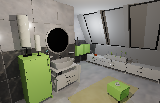
\includegraphics[width=.96\linewidth]{navigation-light/baked/after.png}
\end{minipage}\hfill
\begin{minipage}[c]{.55\linewidth}\centering
{\smalltable\begin{tabular}{@{}lrr@{}}\toprule
第 24 帧的 GPU 调用 & 旧版 & 新版\\\midrule
计算光照和面板颜色 & 4 & 0\\
绘制场景网格 & 85 & 85\\
绘制编辑器界面 & 22 & 22\\\bottomrule
\end{tabular}}
\end{minipage}
\caption{左图从新版事件 510 读取，当时 ImGui 正在显示这张浴室贴图。旧版事件 558 读到的也是这幅图。两份原图均为 $160\times103$，表中每一项按实际 GPU 命令计数。}
\end{figure}

两版均用全部点光源加上烘焙 DDGI。关闭 TAA、GTAO、SSR 和快速导航后，以同一机位运行正式 Vulkan 编辑器。旧版在事件 11 计算直接光，23 读取烘焙探针给表面补光，35 将两者相加，47 把颜色写进面板图。新版直接让 ImGui 读已经画好的贴图。用于鼠标拾取的物体编号仍随场景网格绘制，界面也照常响应。

\begin{figure}[H]\centering
\begin{tikzpicture}[x=1.98mm,y=1mm,font=\sffamily\footnotesize]
  \fill[Rust] (9,14) rectangle (11,18); \node[right] at (11.8,16){重新计算光照};
  \fill[Teal!40] (32,14) rectangle (34,18); \node[right] at (34.8,16){沿用面板图};
  \foreach \row/\limit/\labelname in {8/32/旧版,1/1/新版}{
    \node[left] at (-1,\row) {\labelname};
    \foreach \i in {1,...,55}{
      \ifnum\i>\limit\relax\def\cellcolor{Teal!40}\else\def\cellcolor{Rust}\fi
      \fill[\cellcolor] (\i-1,\row-1.85) rectangle (\i-.10,\row+1.85);
    }
  }
\end{tikzpicture}
\caption{每格是面板大小稳定后的一帧，从左往右共 55 帧。旧版前 32 帧计算光照，随后 23 帧沿用原图；新版计算 1 帧，余下 54 帧沿用原图。}
\end{figure}

直接对照 ImGui 收到的浮点纹理，16\,480 个像素的红、绿、蓝和透明度逐字节相同。打开 TAA 后，镜头虽然不动，每帧仍会在像素内换个位置取样；另一轮 48 帧的检查中，新版为此保留了 32 帧计算。两份捕获来自 RTX 5070 Ti Laptop GPU、Debug x64、RenderDoc 1.47。这次测的是调用次数与画面，整帧耗时需另作计时。

{\small\color{Muted}截图、两份原帧的校验值及复查命令见 \path{output/profiling/navigation-light/baked/}。\par}
\endgroup
